%%%%%%%%%%%%%%%%%%%%%%%%%%%%%%%%%%%%%%%%%
% Beamer Presentation
% LaTeX Template
% Version 1.0 (10/11/12)
%
% This template has been downloaded from:
% http://www.LaTeXTemplates.com
%
% License:
% CC BY-NC-SA 3.0 (http://creativecommons.org/licenses/by-nc-sa/3.0/)
%
%%%%%%%%%%%%%%%%%%%%%%%%%%%%%%%%%%%%%%%%%

%----------------------------------------------------------------------------------------
%	PACKAGES AND THEMES
%----------------------------------------------------------------------------------------

\documentclass{beamer}
\usetheme{Warsaw}
\usepackage[utf8]{inputenc}
\usepackage{amsmath}
\usepackage{amsfonts}
\usepackage{amssymb}
\usepackage{graphicx}
\usepackage{fontspec}
\newfontfamily\cjkfont{Noto Sans CJK SC} % Or any appropriate font you have
\usepackage{graphicx} % Allows including images
\usepackage{booktabs} % Allows the use of \toprule, \midrule and \bottomrule in tables


%----------------------------------------------------------------------------------------
%	TITLE PAGE
%----------------------------------------------------------------------------------------


\author{David Lanzendörfer (leviathan)}
\institute{\textit{Lanceville Technologies Group Ltd.}}
\title{Libre Silicon} % The short title appears at the bottom of every slide, the full title is only on the title page
\setbeamercovered{transparent} 
\setbeamertemplate{navigation symbols}{} 
%\logo{lsa.png} 
\date{\today} % Date, can be changed to a custom date

\begin{document}

\begin{frame}
\titlepage % Print the title page as the first slide
\end{frame}

%----------------------------------------------------------------------------------------
%	PRESENTATION SLIDES
%----------------------------------------------------------------------------------------

%------------------------------------------------
\section[What]{}
\begin{frame}{What we do}
	\begin{itemize}
        \setlength\itemsep{1em}
		\item We make \textbf{truely free silicon} through an open manufacturing process
		\item Breaking the monopoly of big semiconductor manufacturers
		\item Eliminating the vendor lock-in to big semiconductor manufacturers
		\item Making semiconductor development super quick and inexpensive
	\end{itemize}
\end{frame}
\begin{frame}{What we do}
	\begin{itemize}
        \setlength\itemsep{1em}
		\item Introducing the LSPL (LibreSilicon public license)
		\item Attracting commercial design houses to develop \textbf{free silicon}
		\item Eliminating NDAs\footnote{Non-disclosure Agreements} from hardware design flow
		\item Eliminating hardware back doors
	\end{itemize}
\end{frame}

%------------------------------------------------

%------------------------------------------------
\section[Why]{}

\begin{frame}{Why are we doing this?}
	\begin{itemize}
		\item MPWs\footnote{Multi Project Wafer} cost around 20'000 USD
		\item MPWs take around 2-9 months
		\item All manufacturers want NDAs (some NDAs even have NDAs!)
		\item Your design for a vendor process contains process specific design quirks (also under NDA!)
		\item No manufacturer provides the GDS2 files in order to manufacture the designs in your basement (there is \textbf{no} free silicon yet)
		\item You can't even publish your own designs!
	\end{itemize}
\end{frame}

\begin{frame}
	\frametitle{Imagine you like to manufacture your own chip}
	\begin{itemize}
		\item You're going to a foundry
		\item Signing at least 3 NDAs, one for the PDK\footnote{Process design kit}, one for the standard cell libary and one for purchase details
		\item Invest a lot of money for the layout development and the mask set
		\item And have some reasons to change the Foundry Service\dots
	\end{itemize}
\end{frame}

\begin{frame}
	\centering
	
\includegraphics[width=0.75\textwidth]{youre-fucked.png}
\end{frame}

\begin{frame}
\frametitle{Reasons are}
	\begin{itemize}
		\item The technology is completely different
		\item The standard cells are mostly different
		\item The mask does not leave the foundry
		\item And even do not match another technology in another foundry
		\item Well, you've burned the costs for layout and mask set
	\end{itemize}
\end{frame}

\begin{frame}{Closed silicon market}
	\centering
	\hspace*{-0.3in}
	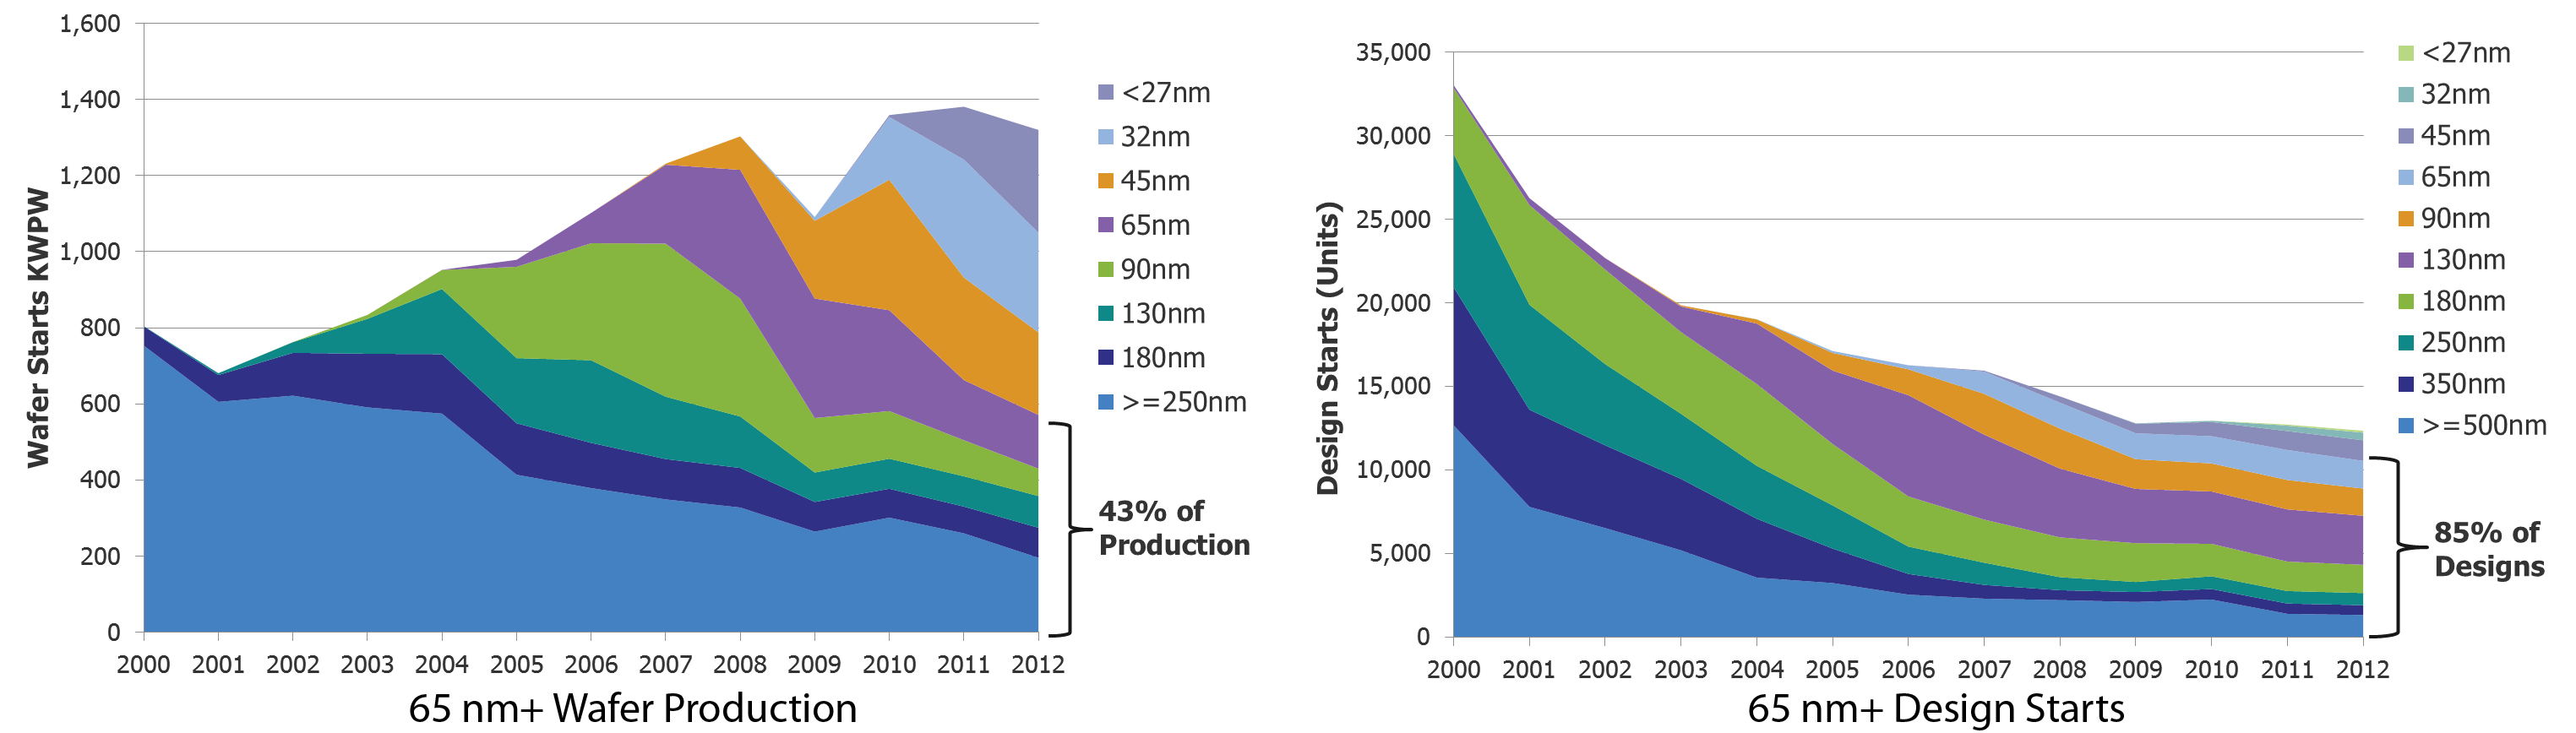
\includegraphics[width=0.75\textwidth]{market-closing.png} \\
	\footnote{http://semimd.com/favre/2016/08/24}
\end{frame}



\section[How]{}

\begin{frame}{How we do it}
	\begin{itemize}
		\item Introducing an open source chip manufacturing process standard specification
		\item Introducing a fully integrated free EDA for ASIC design\footnotemark
		\item Renting the clean room and manufacturing equipment at HKUST every 2 weeks for around 12 hours \\		
		\begin{center}
			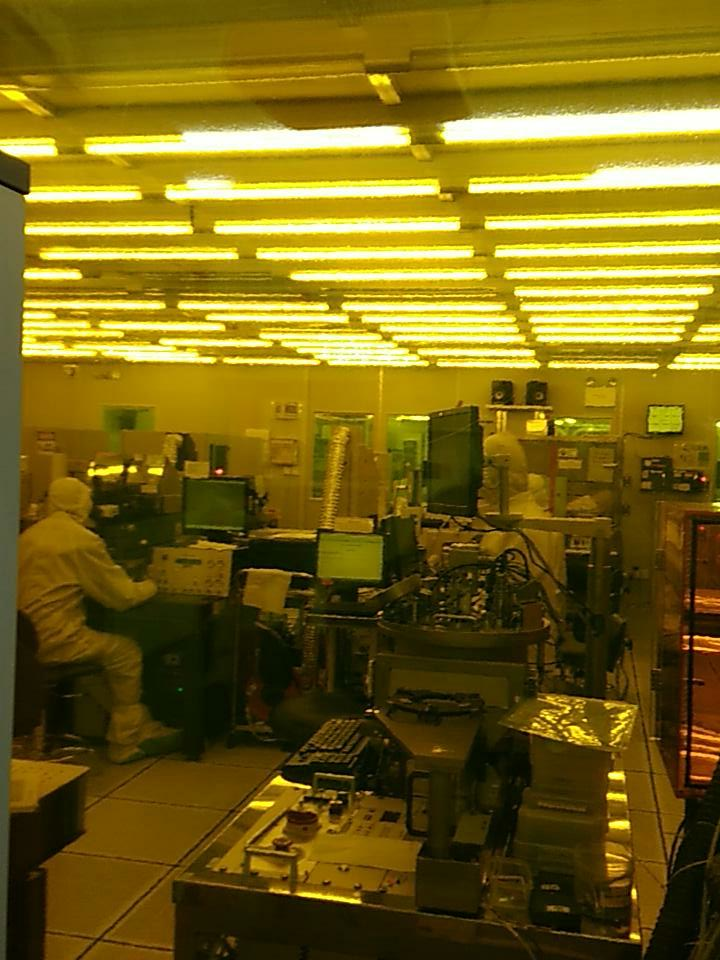
\includegraphics[height=100pt]{cleanroom.png}
			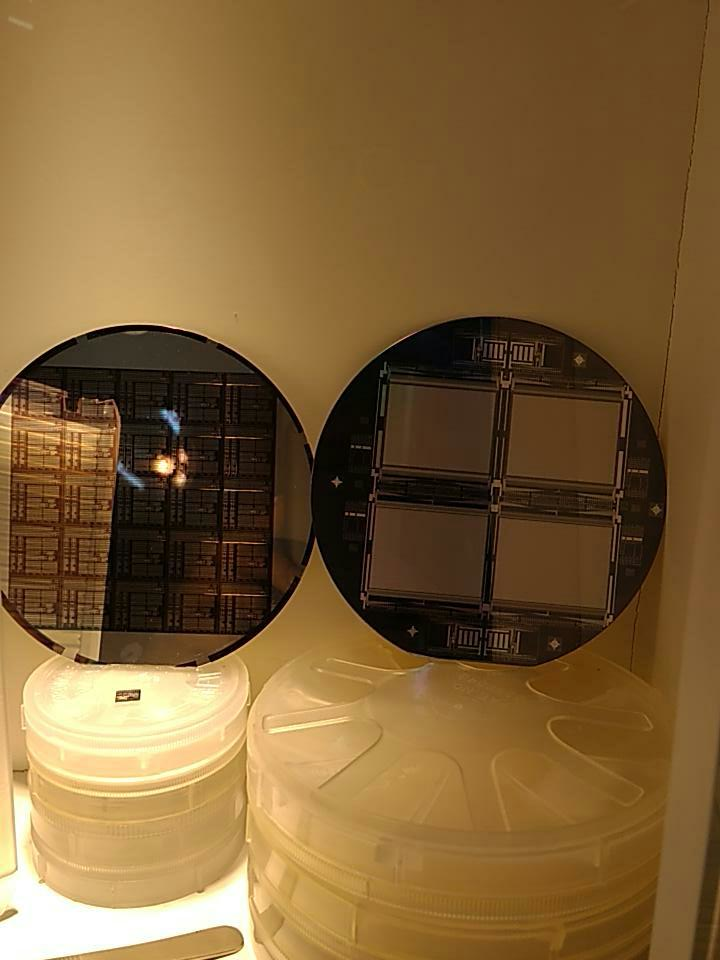
\includegraphics[height=100pt]{examples.png}
		\end{center}
	\end{itemize}

\end{frame}

\begin{frame}{Libre Silicon EDA Tools}
	\begin{itemize}
		\item QtFlow EDA\footnote{\url{https://github.com/leviathanch/qtflow}}
		\begin{itemize}
				\item EDA suite written in Qt5
				\item Wave viewer
				\item Planned:
				\begin{itemize}
					\item Integration of higher level HDLs (CLash)
					\item Plugins through PythonQt
				\end{itemize}
		\end{itemize}
		\item Icarus Verilog simulation\footnote{\url{http://iverilog.icarus.com}}
		\item QRouter maze router\footnote{\url{https://github.com/leviathanch/qrouter}}
		\item GrayWolf floor planner\footnote{\url{https://github.com/leviathanch/graywolf}}
		\item Libre silicon compiler\footnote{\url{https://github.com/foshardware/lsc.git}}
	\end{itemize}

\end{frame}

\begin{frame}
\frametitle{Helpful links}
\begin{itemize}
	\item Mailing list \\
	\url{https://list.o2s.ch/mailman/listinfo/libre-silicon-devel}
	\item Process \\
	\url{https://github.com/libresilicon/libresiliconprocess}
	\item Test wafer (\cjkfont 珠江芯片一号) \\
	\url{https://github.com/chipforge/PearlRiver}
	\item Standard cell library \\
	\url{https://github.com/chipforge/StdCellLib}
	\item Layout software/EDA \\
	\url{https://github.com/leviathanch/qtflow}
\end{itemize}
\Huge{\centerline{You can help :-)}}
\end{frame}

\begin{frame}{PearlRiver (\cjkfont 珠江芯片一号) screen shots}
	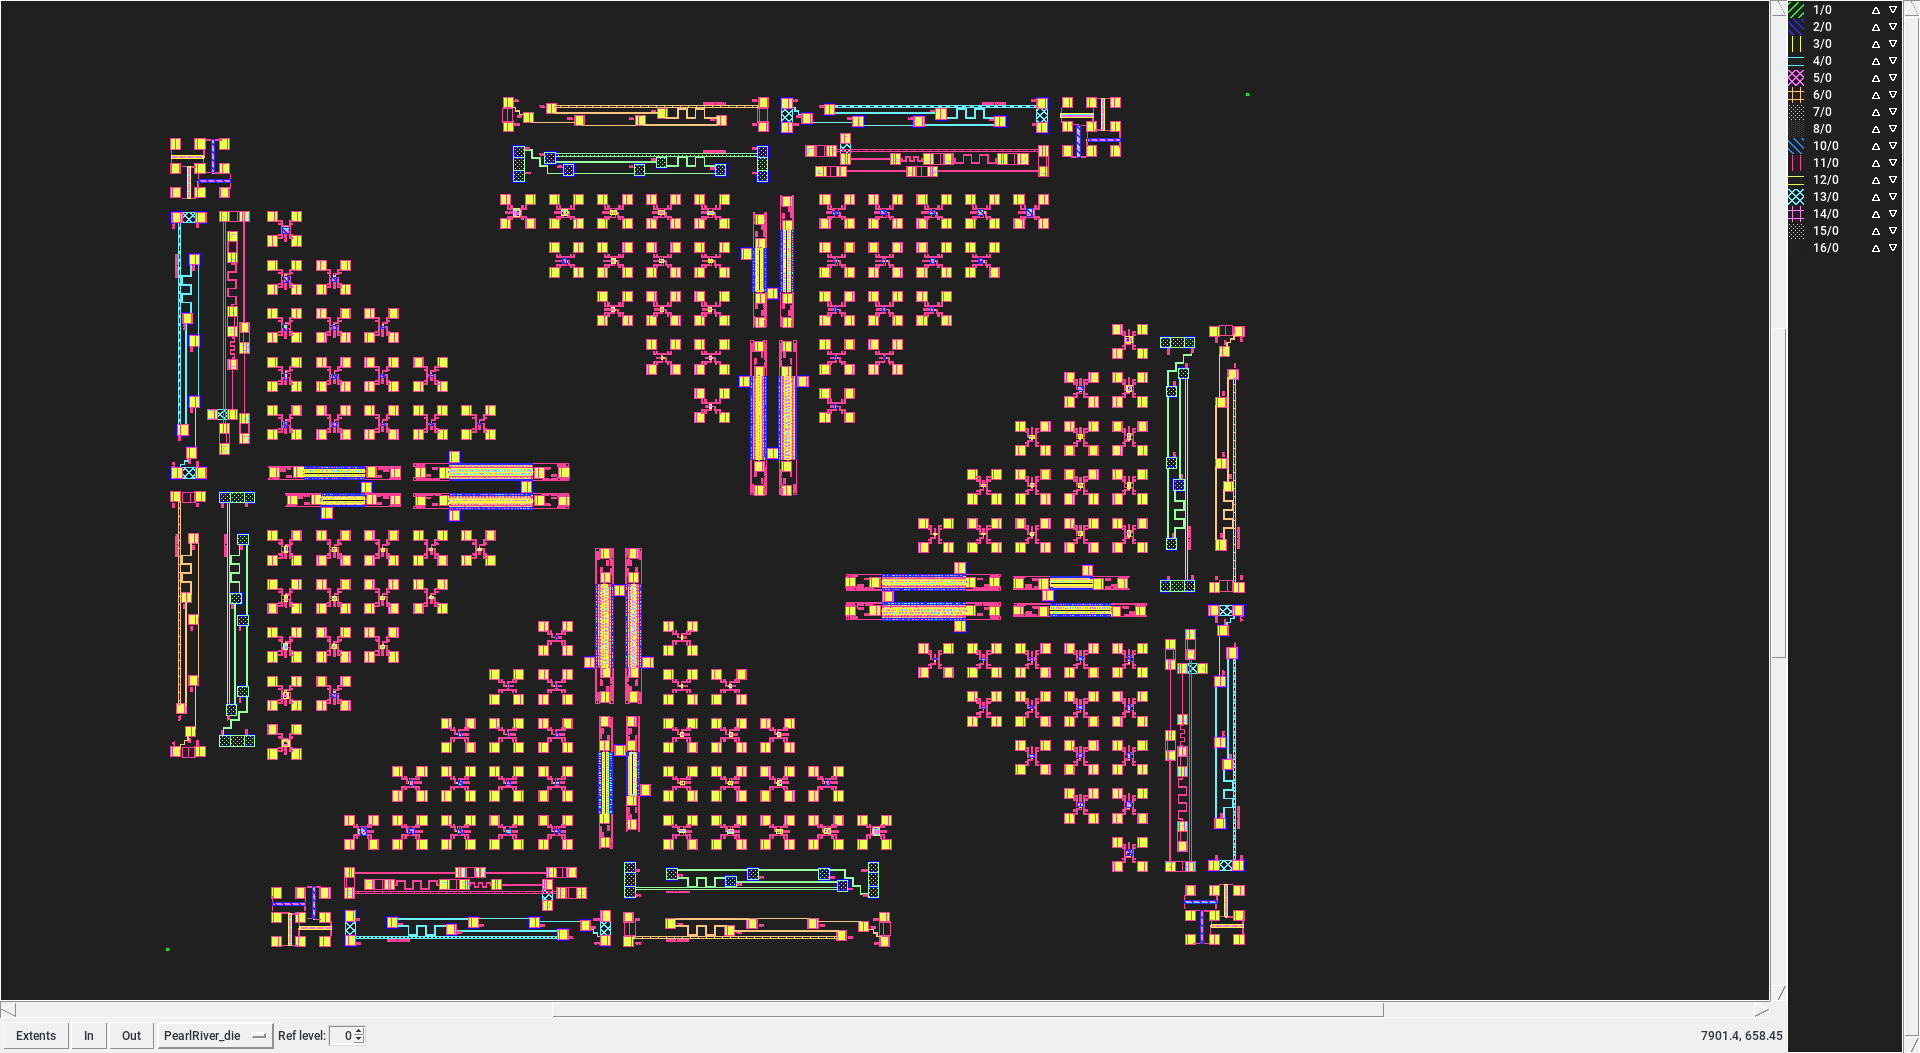
\includegraphics[width=100pt]{Screenshot_20180929_015838.png}\footnote{PearlRiver}
	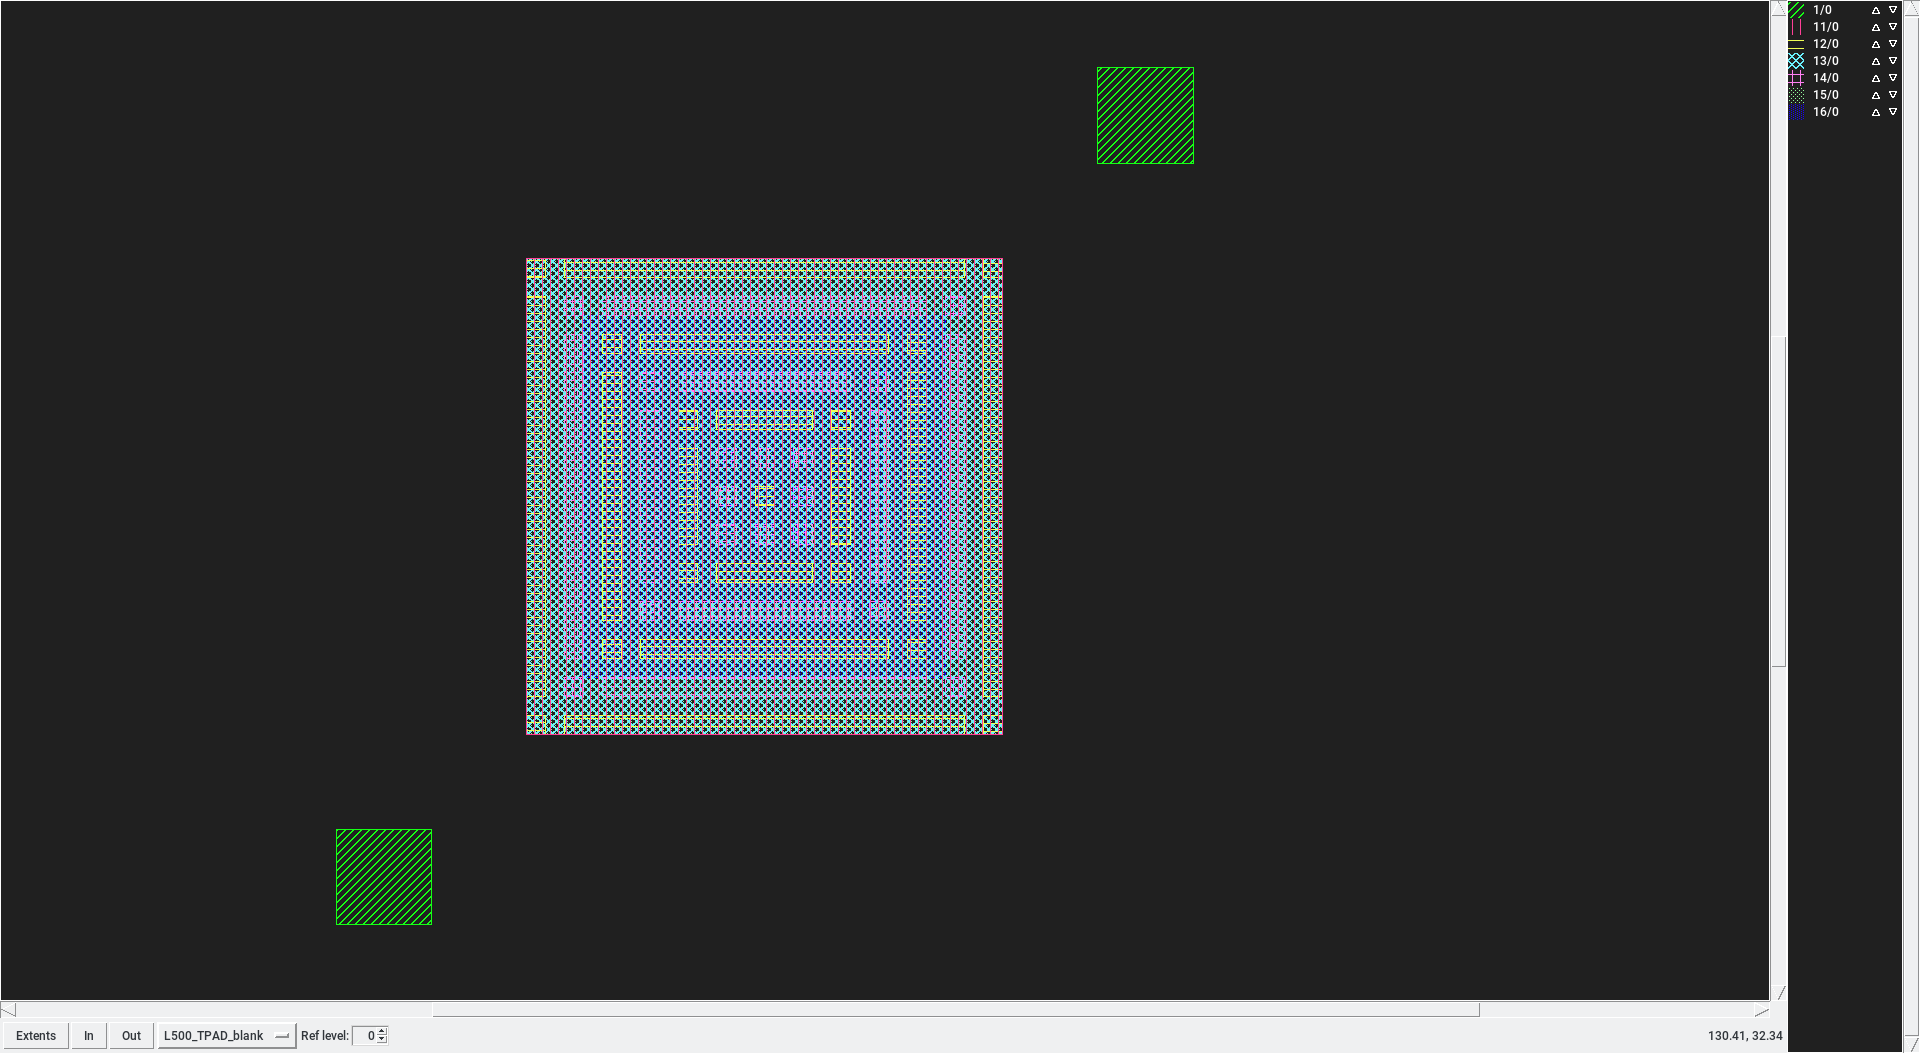
\includegraphics[width=100pt]{Screenshot_20180929_020016.png}\footnote{Bonding pad}
	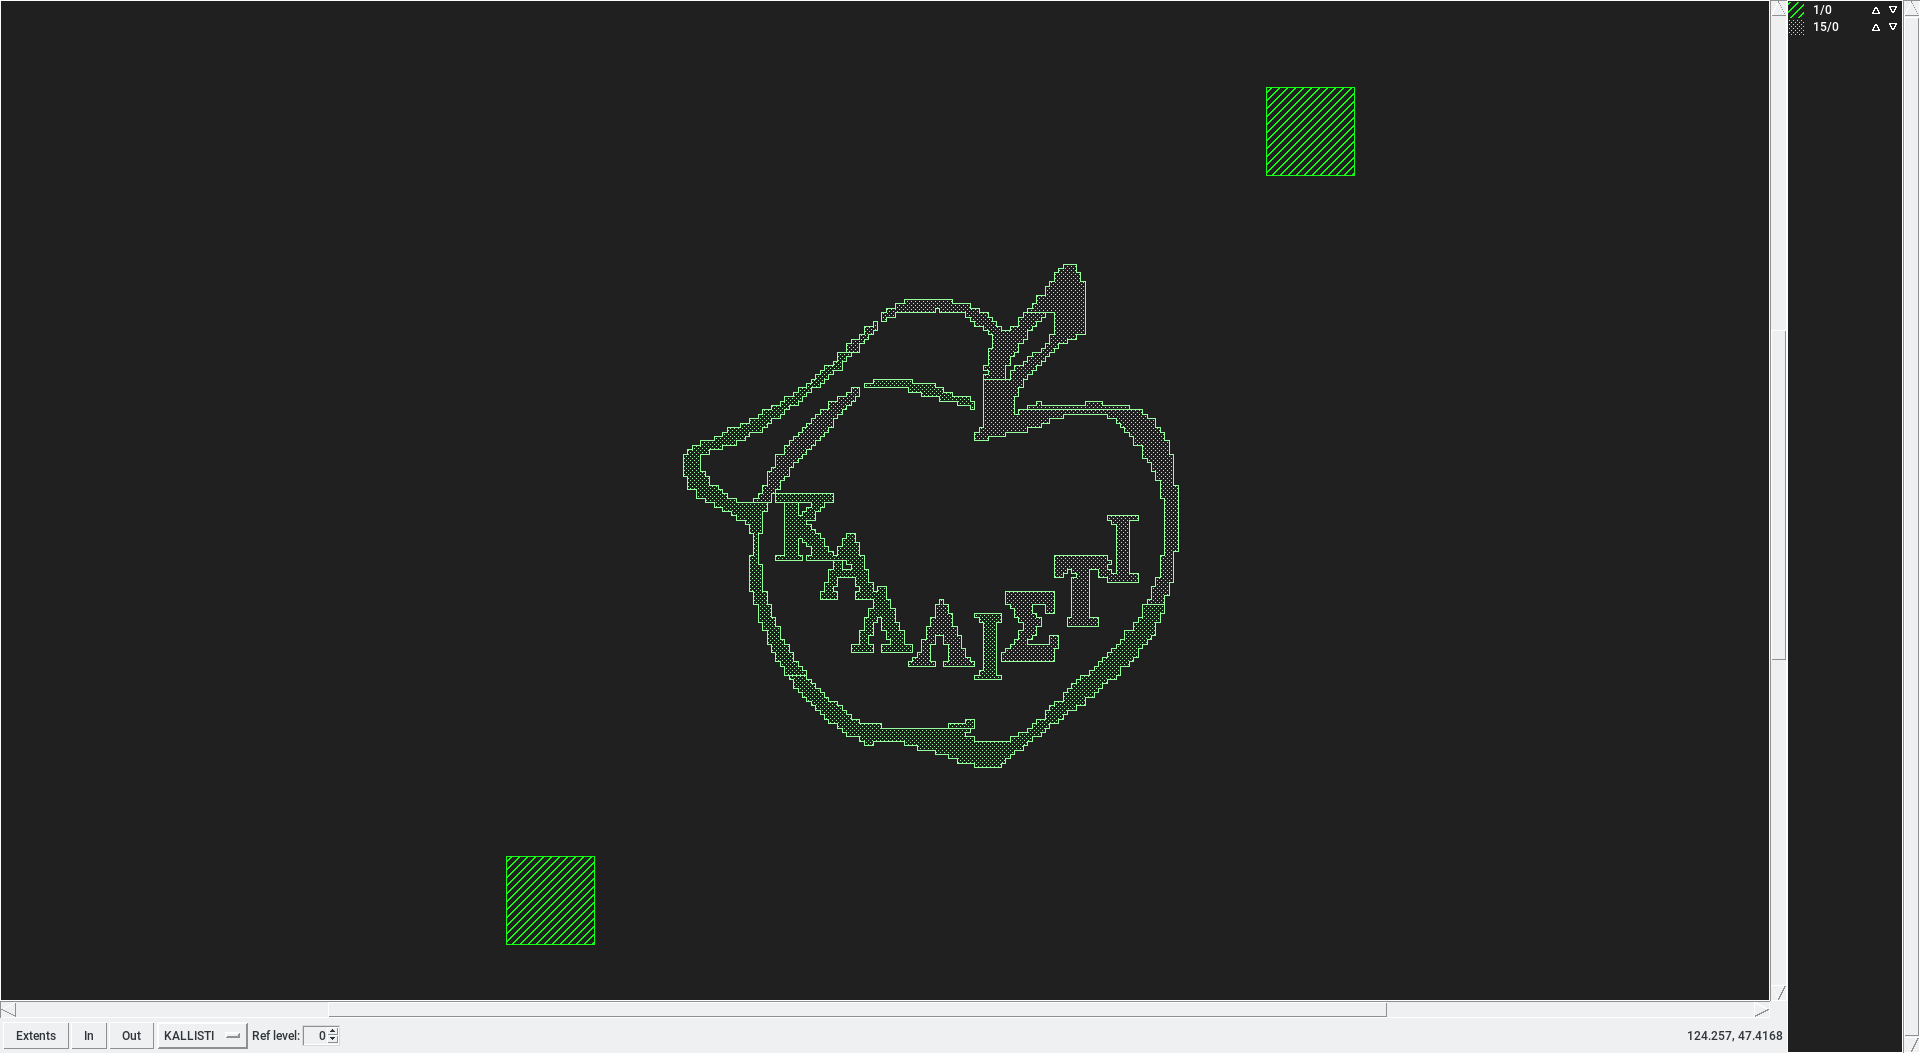
\includegraphics[width=100pt]{Screenshot_20180929_023204.png}\footnote{Holy apple of divine discord}
\end{frame}

\begin{frame}{QtFlow screen shots}
	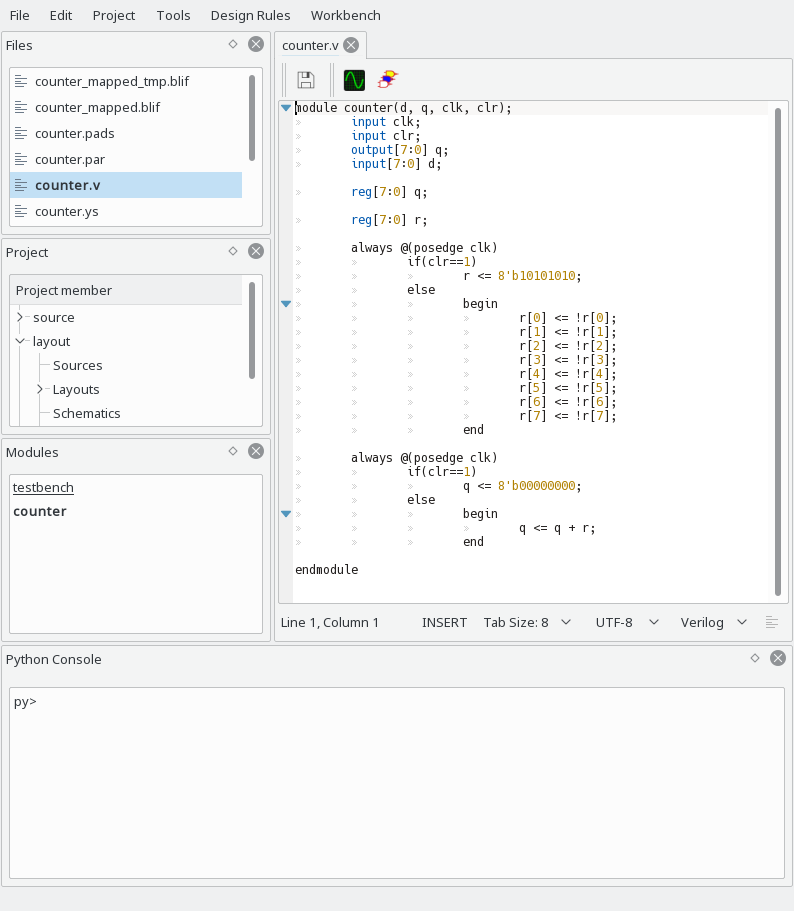
\includegraphics[width=100pt]{Screenshot_20171218_044022.png}
	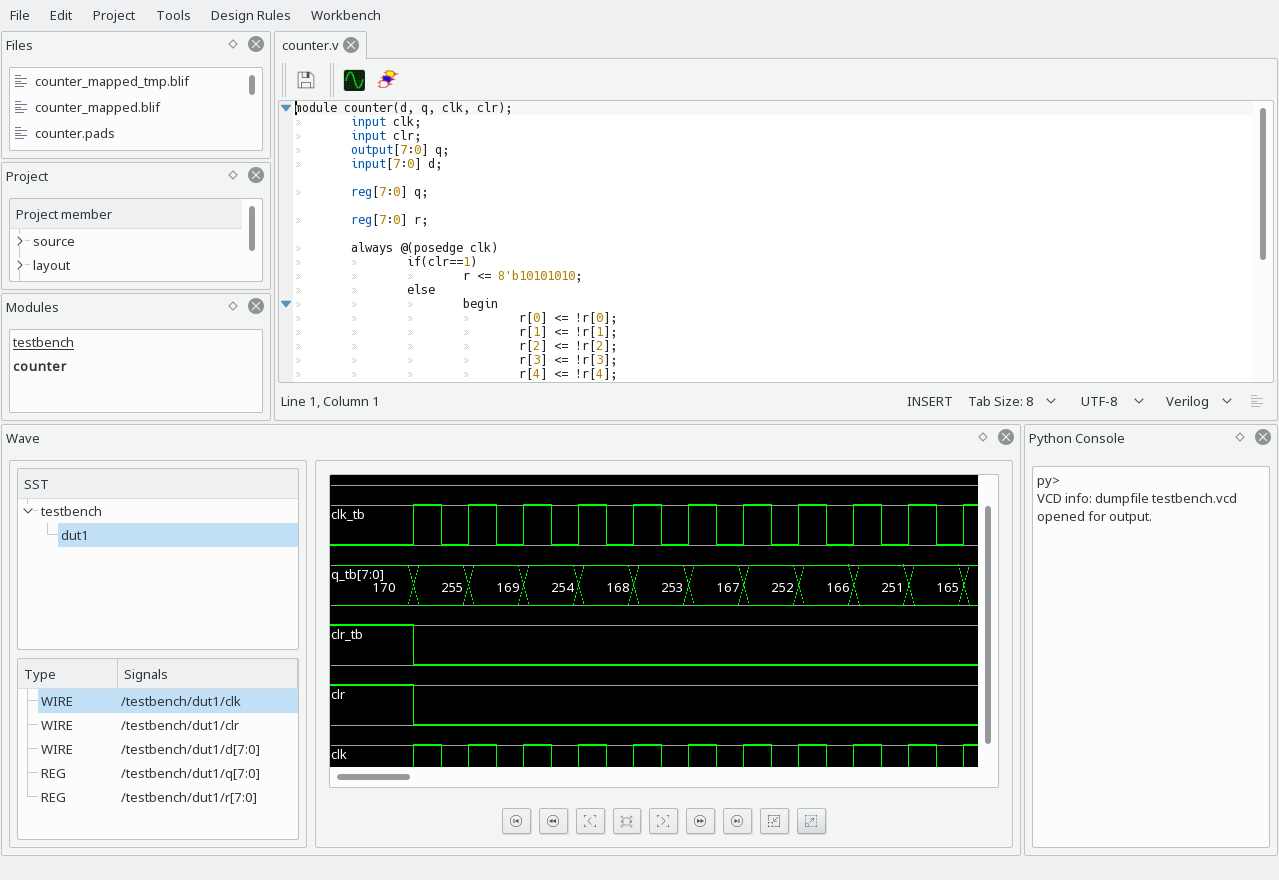
\includegraphics[width=100pt]{Screenshot_20171218_045118.png}
	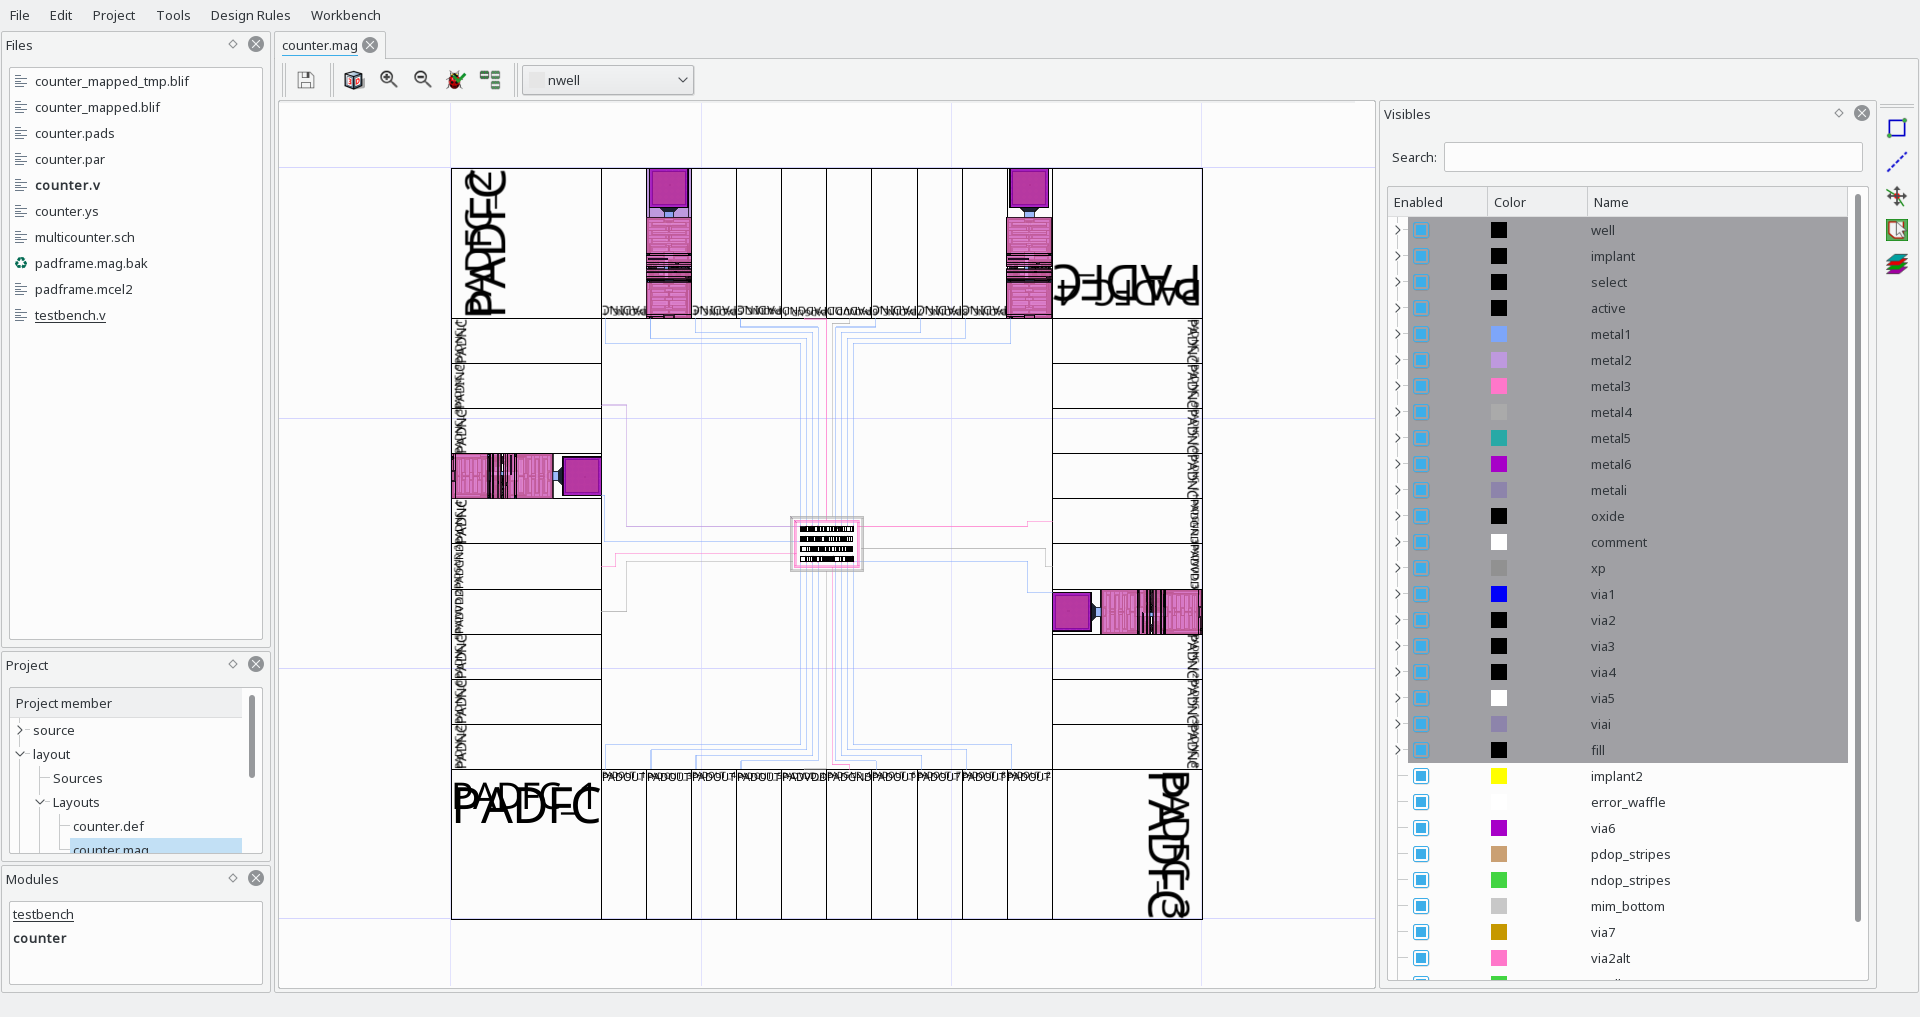
\includegraphics[width=100pt]{Screenshot_20171218_045416.png}
\end{frame}

\begin{frame}
	\frametitle{Make your self independend}
	\begin{itemize}
		\item You know about semiconductor manufacturing? Help us design an open and free process
		\item Fit with licensing? Help us with the LSPL
		\item You can help in other places if you like :-)
	\end{itemize}
\end{frame}

\begin{frame}
	\frametitle{TODO}
	\begin{itemize}
		\item Shrink PearlRiver(\cjkfont 珠江芯片一号) test wafer
		\item Next review before ordering the masks
		\item Documentation about what and how we like to measure parameters
		\item Transfer parameters into Spice BSIM3v3 models
		\item Manufacture a couple of wafers and doing measurement at HKUST
		\item Process refinement
		\item Finish standard cells
		\item Install process foundry for mass production
		\item Manufacture first microcontroller chip in 2019 (\cjkfont 北角芯片)
	\end{itemize}
\end{frame}

\begin{frame}
	\frametitle{License}
	\begin{itemize}
		\item Free and open source - while for real hardware GPL or BSD does not work.
		\item Others like CERN we already evaluated.
		\item We like that everybody can use the process (even in your basement),
		\item Including universities and real foundries.
	\end{itemize}
\end{frame}

\begin{frame}
	\frametitle{Transfer-able}
	\begin{itemize}
		\item Everybody should have the possibility to transfer own designs into other foundries.
		\item Foundries can compete in production cost and / or corporate.
		\item Usable for education also, while even analog designs heavy depends on process parameters.
	\end{itemize}
\end{frame}

\begin{frame}
	\frametitle{The history so far}
	\begin{itemize}
		\item 2017
		\item 2018
	\end{itemize}
\end{frame}

\begin{frame}
	\frametitle{2017}
	\begin{itemize}
		\item leviathan opened a possibility to rent a clean room at Hong Kong University of Science and Technology
		\item leviathan got some funding
		\item leviathan gave a lightning talk in Leipzig at the 34th Chaos Communication Congress
	\end{itemize}
\end{frame}


\begin{frame}
	\frametitle{2018}
	\begin{itemize}
		\item We developed the first version of our 1um LibreSilicon process
		\item We are working on the standard cell library
		\item We already held a tool chain hackathon
		\item We are layouting a first test wafer(\cjkfont 珠江芯片一号) for technology parameter measurement
		\item Currently reviewing the test wafer and compress the layout now for more chips per wafer.
	\end{itemize}
\end{frame}

\begin{frame}
	\frametitle{Links}
	\begin{itemize}
	\item Process \\
		\url{https://github.com/libresilicon/libresiliconprocess}
	\item Test wafer (\cjkfont 珠江芯片一号) \\
		\url{hhttps://github.com/chipforge/PearlRiver}
	\item Standard cell library \\
		\url{hhttps://github.com/chipforge/StdCellLib}
	\item Tool Chain \\
		\url{hhttps://github.com/leviathanch/qtflow}
	\end{itemize}
\end{frame}



\section[Who]{}

\begin{frame}{Community projects}
	\begin{center}
		
\includegraphics[width=100pt]{Icarus.png} \\
		
\includegraphics[width=100pt]{Yosys.png} \\
		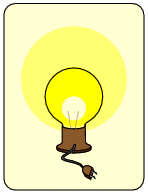
\includegraphics[height=50pt]{Opencircuit.png}
	\end{center}
\end{frame}

\begin{frame}{Companies and institutions}
	\begin{center}
		
\includegraphics[width=100pt]{HKUST_Logo.png}
		
\includegraphics[width=100pt]{NFF.jpg}  \\
		
\includegraphics[width=100pt]{efabless_logo.png} \\
		
\includegraphics[width=100pt]{Lanceville.png}
	\end{center}
\end{frame}



\section[Conclusion]{}

\begin{frame}
	\frametitle{Mumble}
	\begin{itemize}
		\item Weekly voice only conference call over Mumble\footnote{\url{https://www.mumble.com/mumble-download.php}}
		\item Every Sunday 21 p.m Hong Kong Time
		\item Server 109.109.202.102, Port 64738
	\end{itemize}
\end{frame}


\begin{frame}
	\frametitle{Contact me}
	\begin{itemize}
		\item E-Mail (preferred): david.lanzendoerfer@lanceville.cn
		\item Check whether I'm hanging around in Mumble (WARNING: Sometimes there are strange people there, it's public)
		\item IRC: \begin{itemize}
			\item Channel \#\#lsa on irc.freenode.net belongs to LibreSilicon alliance
			\item I'm hanging around on irc.freenode.net as leviathanch
		\end{itemize}
	\end{itemize}
\end{frame}


\begin{frame}{Thanks!}
	\begin{center}
		\textbf{\cjkfont 非常感谢你们!} \\
		\textbf{Thank you very much!} \\
		
\includegraphics[width=100pt]{cat.png}
	\end{center}
\end{frame}

%----------------------------------------------------------------------------------------


\end{document}
